\section{Link Layer}
\label{sec:link}

Two half-duplex stations form \emph{two directed links}, each governed
by its receiver --- only the receiver knows its own noise floor.  There
is no shared ``link mode'' to negotiate; each side requests what it can
hear.

\subsection{The Rate Ladder}

Thirteen operating points (mode $\times$ modulation $\times$ code
rate, dominated rungs removed) span \textbf{7.8--1059\,bit/s} over
\textbf{$-17.9\ldots+4.7$\,dB} (Table~\ref{tab:ladder}).  Every
sensitivity is measured, not derived
(\texttt{experiments/ladder\_sweep.py}, 48 packets/point, recalibrated
receiver; full PER curves in \texttt{results/ladder\_recal.json}).
Requests and grants are ladder indices carried in the link-control
word.  One quirk is documented: rung 1 (ROBUST BPSK 1/3) is dominated
by rung 2 (faster, equally sensitive) and is kept only for
ladder-index stability --- it is never selected.

\begin{table}[H]
    \centering
    \caption{The measured rate ladder (PER $\le 10\,\%$ sensitivities,
             recalibrated receiver, 6\,kHz-band SNR).}
    \label{tab:ladder}
    \small
    \begin{tabular}{@{}rlrr@{\hspace{2em}}rlrr@{}}
    \toprule
    \# & \textbf{mode/mod/FEC} & \textbf{bit/s} & \textbf{dB} &
    \# & \textbf{mode/mod/FEC} & \textbf{bit/s} & \textbf{dB} \\
    \midrule
    0 & EXTREME BPSK 1/3 & 7.8 & $-17.9$ & 7  & NORMAL QPSK 1/2  & 353  & $-5.3$ \\
    1 & ROBUST BPSK 1/3  & 31  & $-11.7$ & 8  & NORMAL QPSK 2/3  & 471  & $-3.8$ \\
    2 & ROBUST BPSK 1/2  & 46  & $-11.8$ & 9  & NORMAL QPSK 3/4  & 529  & $-2.2$ \\
    3 & ROBUST QPSK 1/3  & 62  & $-11.3$ & 10 & NORMAL QAM16 1/2 & 706  & $+0.7$ \\
    4 & NORMAL BPSK 1/3  & 118 & $-7.6$  & 11 & NORMAL QAM16 2/3 & 941  & $+2.6$ \\
    5 & NORMAL BPSK 1/2  & 176 & $-7.3$  & 12 & NORMAL QAM16 3/4 & 1059 & $+4.7$ \\
    6 & NORMAL QPSK 1/3  & 235 & $-7.0$  &    &                  &      &         \\
    \bottomrule
    \end{tabular}
\end{table}

\subsection{The Link-Control Word}

Every frame --- data, ACKs, everything --- piggybacks a 20-bit word in
\texttt{Data.reserved}:
\texttt{seq(2)\,|\,ack(2)\,|\,req\_rung(4)\,|\,snr\_report(4)\,|\,%
freq\_corr(5)\,|\,flags(3)}.  The SNR report uses 2\,dB steps; the
frequency-correction field carries $\pm 120$\,Hz in 8\,Hz steps
(Section~\ref{sec:afc}); flags are last-fragment, no-data (ACK-only),
and priority-stream.

\subsection{Rate Adaptation: Three Feedback Paths}

Figure~\ref{fig:adaptation} shows the controller.  On the receive
side, per-frame SNR estimates pass through a fade-aware filter (the
second-lowest of recent measurements, age-windowed to 60\,s) before
driving the rung request: upshift requires the target rung's
sensitivity plus 2.5\,dB of held margin, downshift triggers below
1\,dB (the hysteresis band prevents ping-pong), and inbound
\emph{silence} decays the request and purges the measurement history
--- without the purge, stale pre-fade measurements resurrect a high
rung the moment one frame gets through.

\begin{figure}[H]
    \centering
    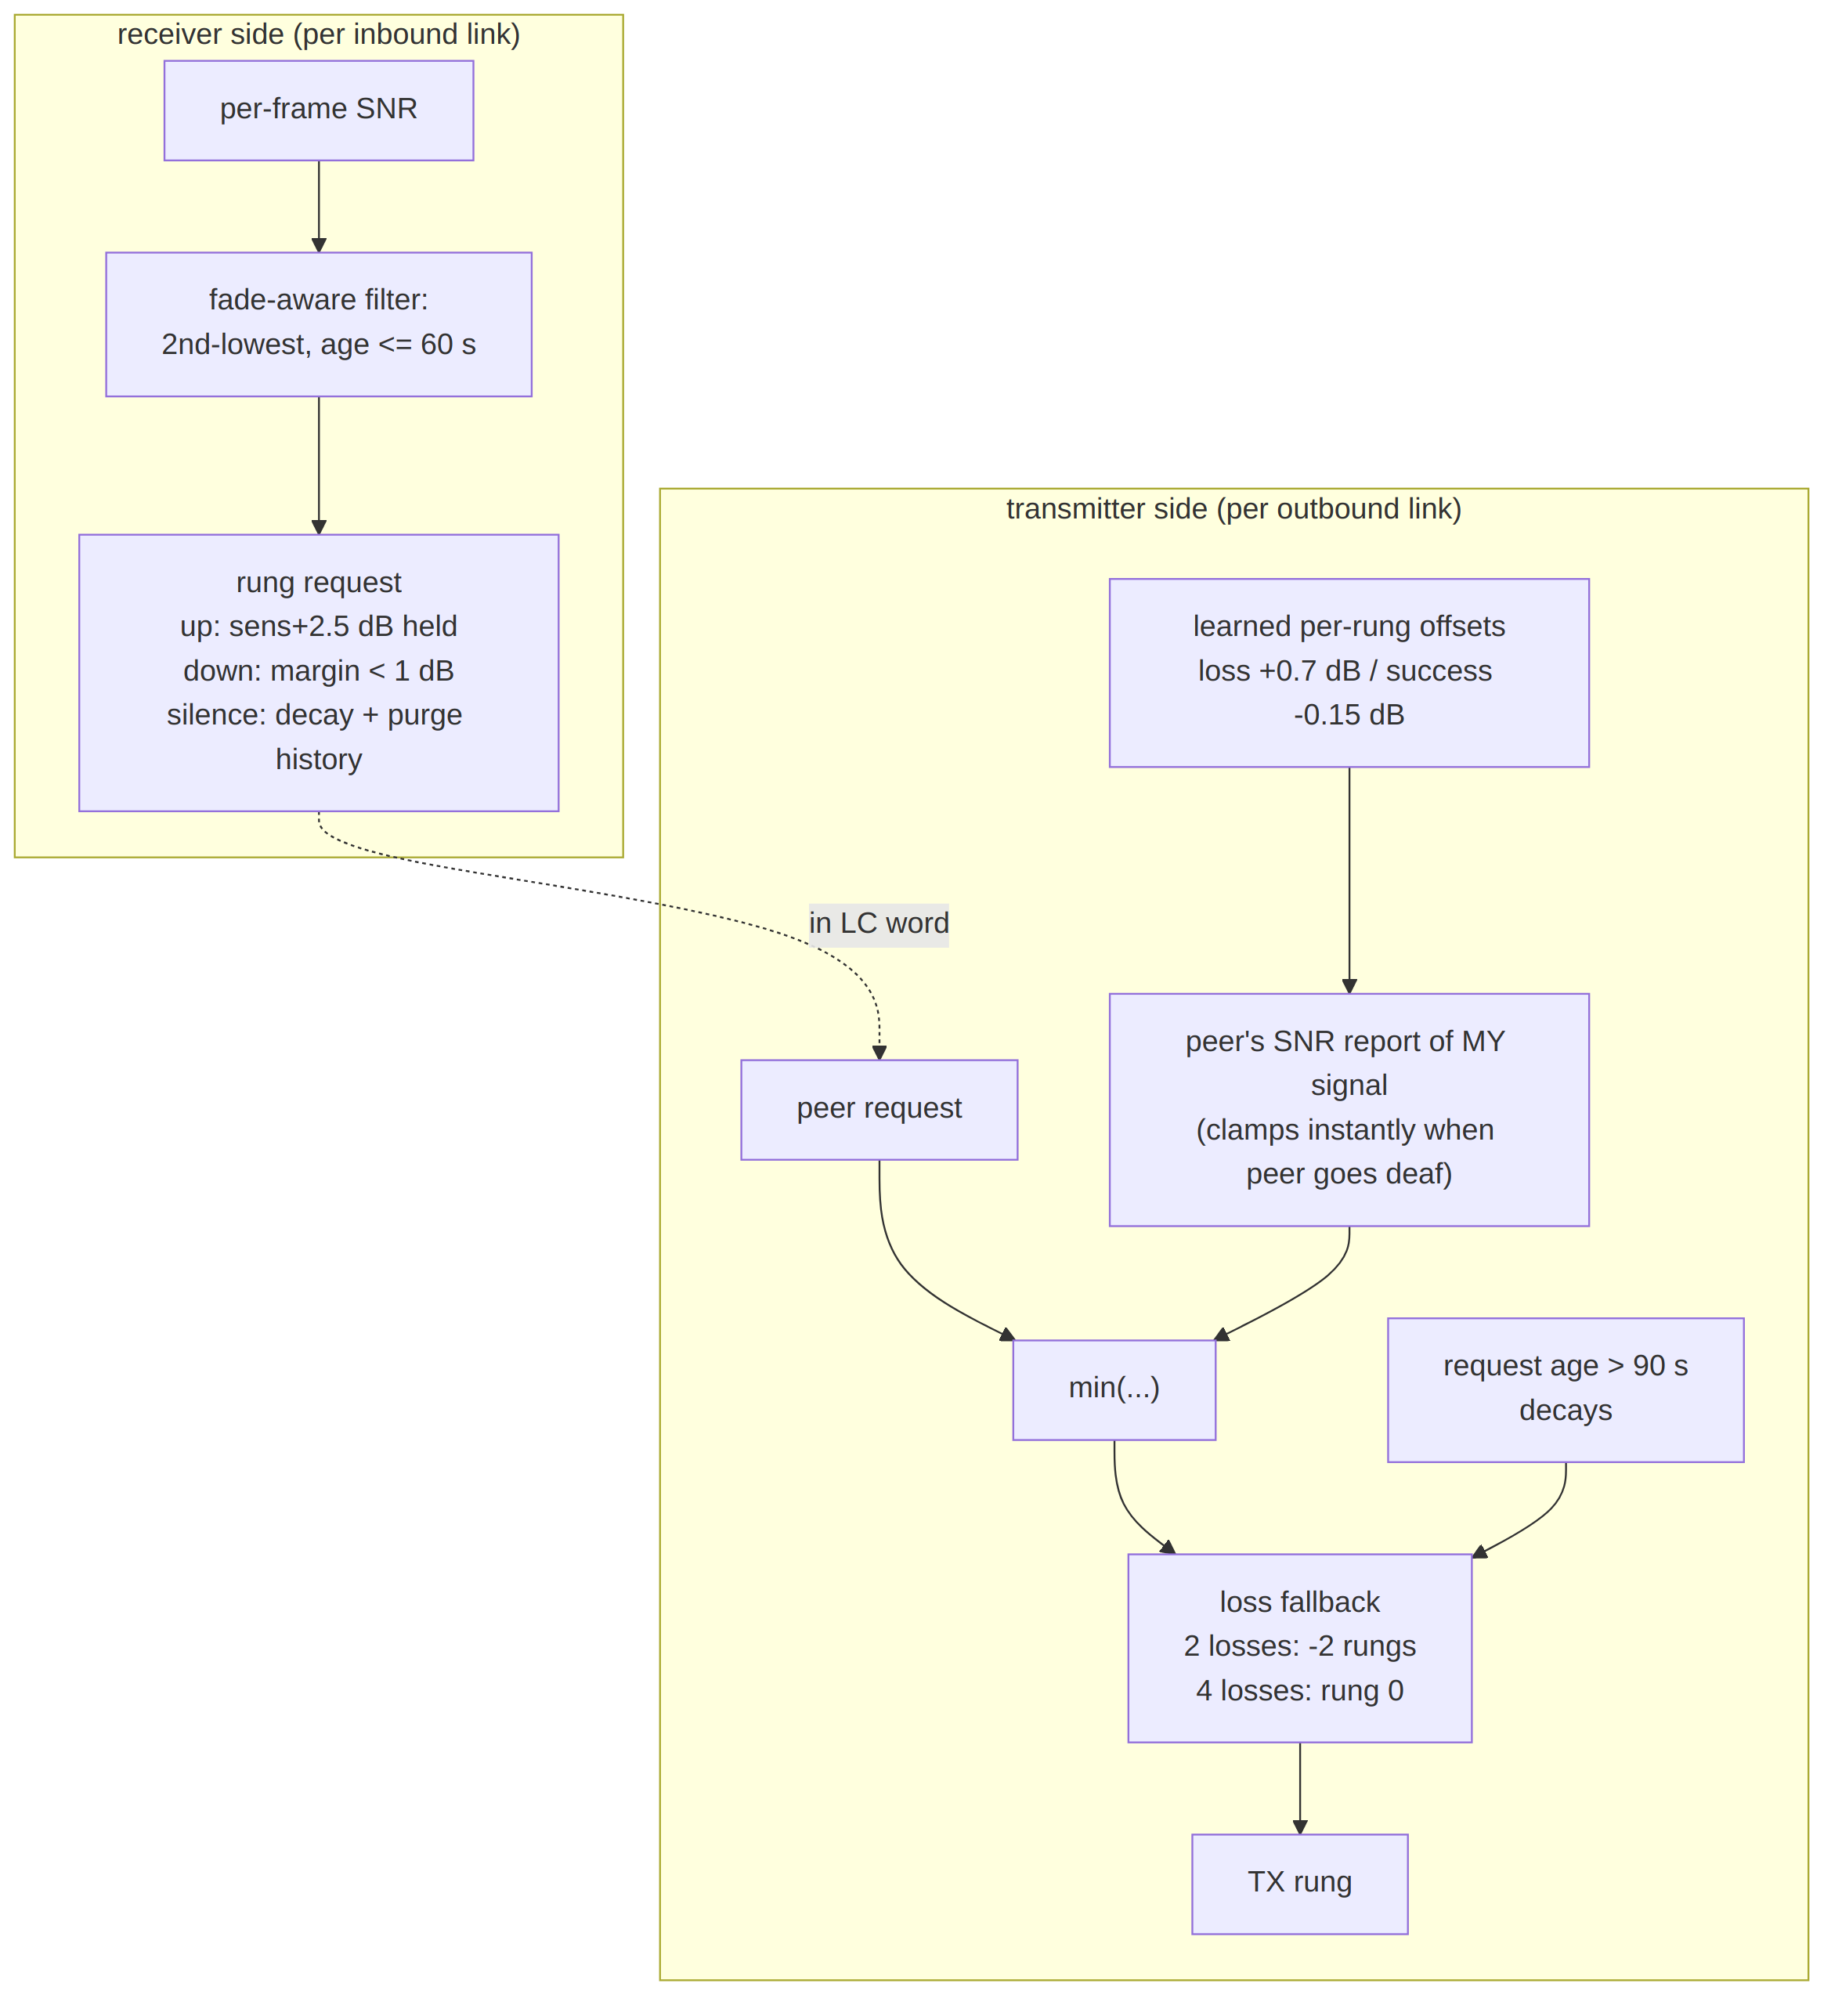
\includegraphics[width=\textwidth]{images/adaptation.png}
    \caption{Receiver-driven rate adaptation.  The three feedback paths
             have three different latencies: the peer's explicit
             request (one round trip), the peer's SNR report of
             \emph{your} signal (instant clamp when the peer goes
             deaf), and loss-driven fallback (no feedback at all).}
    \label{fig:adaptation}
\end{figure}

On the transmit side, the rung is the minimum of the peer's request
and a cap derived from the peer's SNR report of our own signal,
adjusted by \emph{learned per-rung offsets} ($+0.7$\,dB on loss,
$-0.15$\,dB on success --- correcting the static table per
deployment), with loss fallback (2 consecutive losses
$\rightarrow -2$ rungs, 4 $\rightarrow$ rung 0) and staleness decay.
Bootstrap is trivial by construction: both sides start at rung 0
(EXTREME), which works whenever anything works, and one decoded
exchange carries enough measurement to jump directly to the
SNR-indicated rung.

\subsection{ARQ, QoS, and Preemption}

ARQ is stop-and-wait with piggybacked ACKs (the 2-bit sequence number
suffices), enhanced by the HARQ combining of Section~\ref{sec:coding}.
An invariant worth recording: sequence numbers 0--7 are all
legitimate, so ``nothing received yet'' is represented by
\texttt{None}, never a magic value --- the initial implementation used
7 as a sentinel and deadlocked the moment a real frame carried
sequence 7.

QoS is policy, not machinery: three classes (control $>$ interactive
$>$ bulk) with strict priority; per-class air-time caps size fragments
(a 27-byte EXTREME frame is 43\,s of air time, so latency budgeting
happens at segmentation); control and ACK traffic rides one rung below
bulk for extra margin.  The priority stream \emph{preempts} an
in-progress bulk message at fragment boundaries --- the
priority-stream LC flag selects one of two reassembly buffers --- so
an urgent message injected mid-transfer arrives $\sim$23\,s before the
bulk completes instead of after it.

\subsection{Burst Windows and Streaming}
\label{sec:burstwin}

Bulk transfers use selective repeat: a window of fragments goes out
back-to-back, answered by one bitmap acknowledgment
(NACK-by-omission).  Where the PHY offers streaming
(Section~\ref{sec:stream}), the whole window is sent behind a
\emph{single} preamble and header rather than one preamble per
fragment.  The packets are byte-identical to per-frame burst fragments
--- one spare bit in the sub-header's index byte marks a fragment as
streamed --- so a receiver without streaming support still decodes the
first block of every burst as an ordinary fragment.  That property is
what makes the fallback safe rather than fatal.

The window is chosen once, at engage, as
$\min(\text{operator ceiling}, \text{buffer cap},
\text{fragment count})$, then clipped by an air-time cap so that a
single transmission can never outlast a plausible fade --- everything
in a streamed window is exposed before any of it is acknowledged.
Sizing the window to the transfer is what makes a short transfer cost
exactly one acknowledgment, which is the deferred-NAK arrangement of
LTP and CFDP arrived at through a constant rather than new wire
format.  Measured on a 14\,kB file over the virtual channel: window 4
takes 14 transmissions, window 8 takes 9, window 16 takes 6.

Resizing the window \emph{during} a transfer was implemented and then
reverted on the evidence.  Halving it on each streamed-window timeout,
rather than striking out of streaming, collapsed the window
$16\to8\to4\to2\to1$ with no path back --- it grows only on a fully
acknowledged window, which never happens inside a fade --- and produced
196 transmissions with 72 timeouts against 134 and 9 for the
strike-out path.  On a clean channel the two were indistinguishable.
When a fade is what breaks a burst, the correct response is to stop
streaming, not to stream less.

Three conditions end streaming for a transfer, and they are not the
same kind of statement.  A bitmap that acknowledges at most one
fragment of a window of three or more is the signature of a peer
decoding only the first block: that is a statement about the
\emph{peer}, and it is remembered across transfers, because a receiver
unable to follow a stream will not learn to between them.  Repeated
timeouts and a transmitter-side build refusal describe the
\emph{channel} and the local buffers respectively, and deliberately do
not stick --- a fading channel raises timeouts against a peer that
streams perfectly well, and making that sticky would disable streaming
for the session on a capable link.  The peer verdict is not permanent
either, since a deep fade can forge the one-fragment signature:
streaming is probed again after eight transfers, which bounds a wrong
verdict to one wasted window per retry period while a genuinely
incapable peer costs two windows per period instead of two per
transfer.

\subsection{The Reply Timer}
\label{sec:rto}

A station that has transmitted and expects an answer must decide how
long to wait.  The budget splits along what is knowable.  The reply's
\emph{air time} is computable exactly from the rung and the expected
reply length, and it swings by a factor of forty across the ladder, so
smoothing it would be meaningless.  Everything else --- the peer's
turnaround, its decode time, its wait for the channel to clear, its
scheduling, and the error in our guess of which rung it will answer at
--- is latency that can only be measured.

The air term is therefore computed and the overhead is estimated in
the manner of RFC~6298: a smoothed mean and variance
($\alpha = 1/8$, $\beta = 1/4$) with the budget set at
$\text{srtt} + 4\,\text{rttvar}$.  Karn's rule keeps ambiguous
exchanges out of the estimator --- a reply that follows a
retransmission cannot be attributed to a particular transmission ---
and a timeout doubles the timer until a clean exchange clears the
backoff.  Against a peer that consistently takes 0.40\,s, the
2.30\,s bootstrap guess converges to 0.40\,s.

This replaces a fixed margin that had already caused a
misdiagnosis. When the host could not sustain the demonstration
harness's 25$\times$ time compression, the two stations' sample-derived
clocks drifted apart --- the mostly-transmitting station stayed
current while the one decoding three receivers fell behind --- and the
transmitter timed out before the receiver had finished the burst in
its own timeline.  Every timeout landed on one station and none on the
other, with the reply arriving immediately after each: a signature
that reads exactly like a protocol failure and is not one.

\subsection{Simplex Channel Access}

Both stations share one frequency and are deaf while transmitting.
Figure~\ref{fig:simplex} shows the access state machine.  The
load-bearing rules: carrier sense before keying; the listen window is
sized from the \emph{expected reply's} air time at the peer's rung; a
timeout on a \emph{busy} channel is not a loss (the peer may be
replying at a slower rung); random 1--6\,s backoff breaks the symmetry
of two stations keying together; and a station replies only to frames
that carried data --- no ACK-of-ACK loops.

\begin{figure}[H]
    \centering
    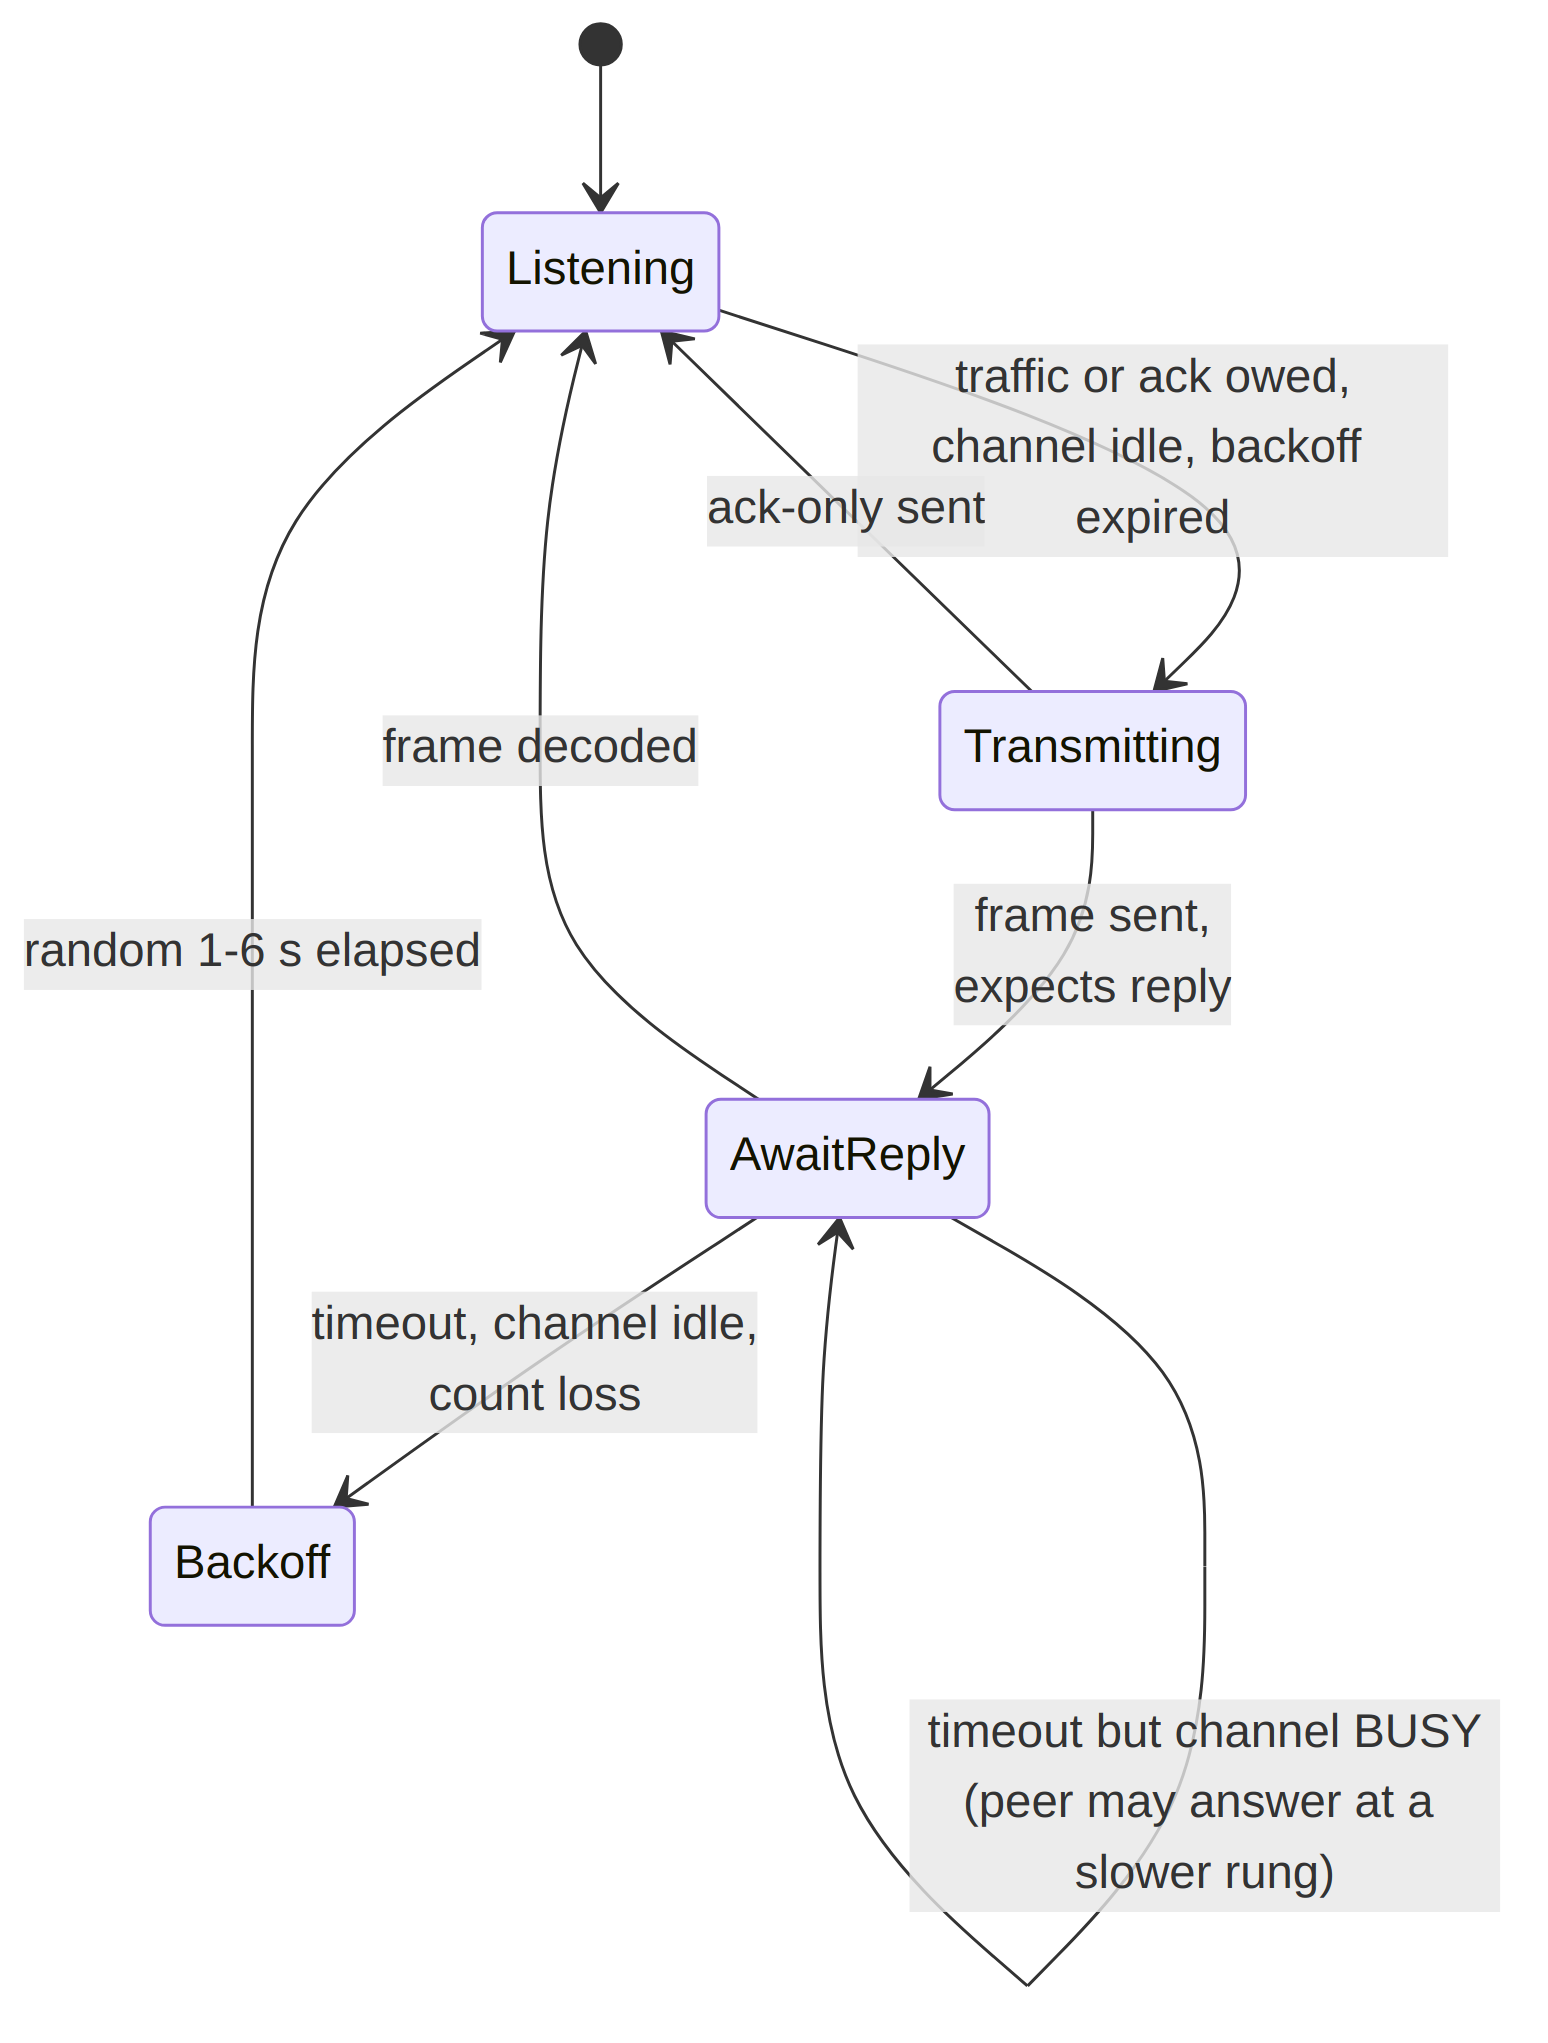
\includegraphics[width=0.85\textwidth]{images/simplex_state.png}
    \caption{Simplex channel-access state machine
             (\texttt{LinkStation.poll\_tx}).}
    \label{fig:simplex}
\end{figure}

The whole-system test (\texttt{experiments/simplex\_session.py}) runs
two stations with bidirectional QoS traffic and a $-14$\,dB fade in
the middle of the bulk transfer: all messages deliver bit-exact in QoS
priority order, the fade costs four timeouts and one
fallback-and-recover cycle, and the session terminates without
deadlock at 11--22\,bit/s effective on the shared channel.
Figure~\ref{fig:link_adaptation} shows the controller-level
simulation: bootstrap at EXTREME, a fast climb to the QPSK rungs,
loss-driven fallback within two frames of a sudden fade, and
recovery.

\begin{figure}[H]
    \centering
    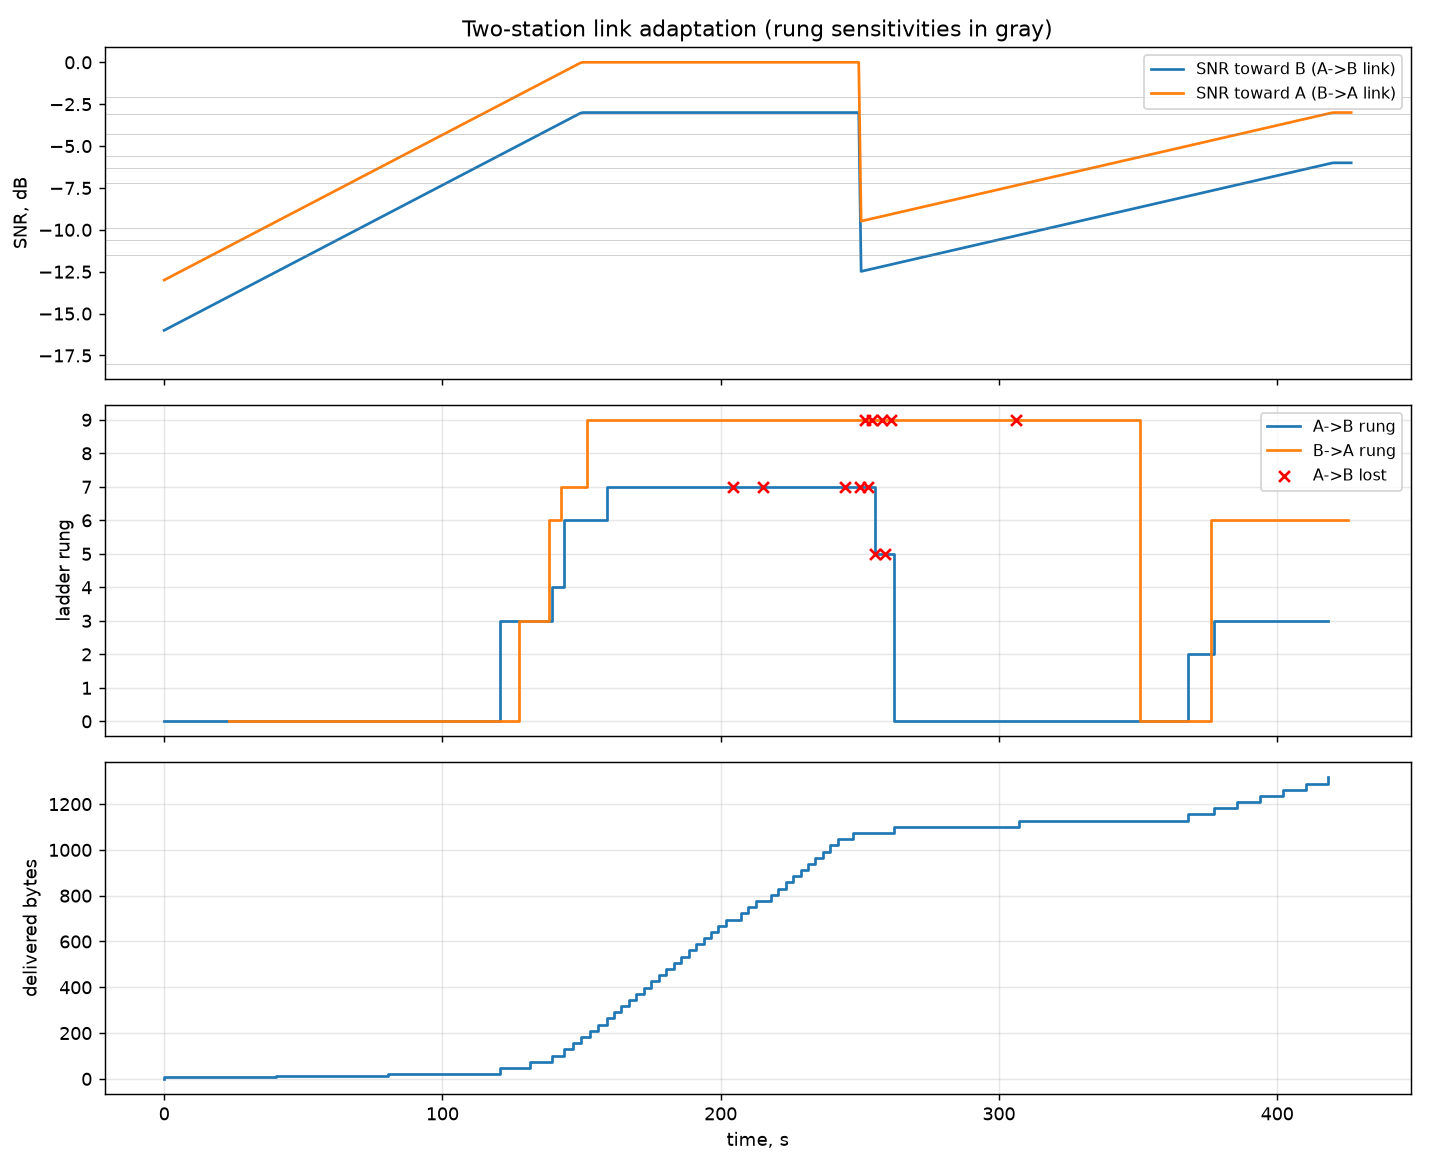
\includegraphics[width=\textwidth]{images/link_adaptation.png}
    \caption{Controller-level two-station simulation
             (\texttt{experiments/link\_adaptation.py}): asymmetric
             channel, $-16$\,dB start, sudden fade; 1290/1500 bytes
             delivered at 24\,bit/s effective goodput including ACK
             overhead and turnarounds.}
    \label{fig:link_adaptation}
\end{figure}
